\chapter{Cordes longues et correspondance avec les trous noirs}

\lectureoverview{Un trou noir possède une entropie ; il doit donc avoir des degrés de liberté microscopiques. Nous allons élaborer l’explication la plus simple de ces degrés de liberté dans le cadre de la théorie des cordes : nous commencerons par dénombrer les états d’une corde longue et excitée, puis nous ferons varier le couplage des cordes jusqu’à ce que les descriptions en termes de corde et de trou noir se rejoignent. L’égalité finale est délibérément laissée en exercice pour le cours suivant.}

\section{L’entropie exige des degrés de liberté microscopiques}

Dire qu’un système possède une grande entropie, c’est dire qu’il peut dissimuler une grande quantité d’information microscopique. Une baignoire d’eau chaude peut avoir une entropie de l’ordre de \(10^{30}\). Cela nous indique déjà qu’il existe un très grand nombre de degrés de liberté microscopiques, que nous choisissions ou non de les examiner molécule par molécule. La thermodynamique permet de déterminer l’entropie en mesurant l’énergie et la température, mais elle n’identifie pas les objets qui en sont porteurs.

La mécanique des fluides rend cette distinction familière. Elle décrit la densité, la vitesse, la pression et l’écoulement macroscopique sans faire référence aux atomes. En y ajoutant la thermodynamique, on découvre qu’un fluide possède une entropie. Celle-ci révèle une structure microscopique que les équations à gros grains ne font pas apparaître ; elle invite à poser une nouvelle question au lieu d’y répondre.

Les trous noirs posent le même problème sous une forme plus aiguë. La proposition de Bekenstein, complétée par le calcul de Hawking, attribue une entropie proportionnelle à l’aire de l’horizon. La relativité générale détermine la géométrie et sa thermodynamique, mais ne fournit aucun inventaire des états microscopiques. Quels sont ces objets minuscules et nombreux dont les configurations rendent compte de la loi d’aire ? La théorie des cordes offre un candidat concret. L’argument développé ici est volontairement qualitatif : il donne la bonne dépendance paramétrique tout en négligeant les constantes numériques et les outils formels nécessaires à un dénombrement complet des états.

\section{Trois échelles et un piège de notation}

La gravitation fait intervenir une longueur privilégiée, la longueur de Planck,
\begin{equation}
\ell_p=\sqrt{\frac{G_N\hbar}{c^3}}.
\label{eq:l06-planck-si}
\end{equation}

\begin{classroomqa}
\audiencequestion{Quelle combinaison de \(G_N\), de \(\hbar\) et de \(c\) donne la longueur de Planck ?\lecturetimestamp{00:06:08}}
\lecturerresponse{C’est \(\sqrt{G_N\hbar/c^3}\), soit environ \(10^{-33}\) centimètres. Nous posons aussitôt \(\hbar=c=1\), ce qui simplifie considérablement la relation.}
\end{classroomqa}

En unités naturelles,
\begin{equation}
\hbar=c=1,
\qquad
G_N=\ell_p^2.
\label{eq:l06-planck-area}
\end{equation}
La constante de Newton a donc les dimensions d’une aire. C’est pourquoi une aire divisée par \(G_N\) est sans dimension et peut représenter une entropie.

La théorie des cordes fait intervenir une deuxième longueur, \(\ell_s\). Si l’on chauffe une corde, ou si on la place dans un état très excité, elle oscille à de nombreuses échelles. Dans cette représentation élémentaire, la longueur caractéristique la plus courte est la longueur de corde. On peut considérer \(\ell_s\) comme la taille associée à un quantum élémentaire d’oscillation de la corde.

La troisième quantité est le couplage des cordes sans dimension \(g_s\). Il régit les scissions et les fusions : une corde peut se pincer et se diviser en deux, ou une corde excitée peut émettre un quantum de corde fermée.

\begin{classroomqa}
\audiencequestion{Quelle est la signification physique du couplage des cordes ?\lecturetimestamp{00:09:20}}
\lecturerresponse{Il régit la probabilité d’une interaction entre cordes, par exemple la scission d’une corde qui s’entrecroise. Plus précisément, \(g_s\) est l’amplitude d’interaction ; la probabilité ou le taux correspondant commence à l’ordre \(g_s^2\).}
\end{classroomqa}

L’excitation sans masse de corde fermée émise peut être un graviton. À cet égard, \(g_s\) joue un rôle analogue à celui de la charge électrique : c’est le facteur associé à un sommet d’interaction.\editorialnote{Dans ce cours, \(g_s\) est parfois appelé probabilité et parfois amplitude. En théorie des perturbations, il s’agit du couplage au niveau de l’amplitude ; les probabilités et les taux font intervenir son carré.}

\section{Pourquoi la gravitation dépend du \texorpdfstring{\(g_s^2\)}{carré du couplage}}

Considérons d’abord le schéma d’échange en électromagnétisme. Un objet chargé émet un photon avec un facteur \(e\), et un second l’absorbe avec un autre facteur \(e\). L’amplitude d’échange contient donc \(e^2\). Ce schéma ne décrit pas littéralement un projectile classique, mais il montre correctement comment intervient le couplage.

\begin{figure}[htbp]
\centering
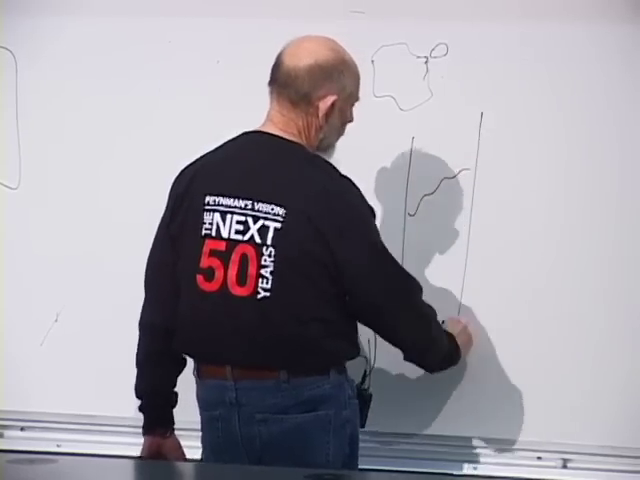
\includegraphics[width=0.72\textwidth]{lecture_06_figure_03.png}
\caption{Le schéma d’échange complété au tableau : un facteur de couplage intervient à l’émission, puis de nouveau à l’absorption.}
\lectureframe{00:11:30.000}
\end{figure}

Dans la version de la théorie des cordes, le graviton remplace le photon et \(g_s\) remplace la charge électrique. Un facteur accompagne l’émission et un autre l’absorption ; l’intensité de l’interaction gravitationnelle est donc proportionnelle à \(g_s^2\).

À grande distance, la même interaction doit reproduire la loi de force de Newton,
\begin{equation}
F_{\mathrm{grav}}\sim G_N\frac{M_1M_2}{r^2}.
\end{equation}
Les masses et la dépendance en l’inverse du carré décrivent les sources et la propagation ; ce qui nous importe ici, c’est le couplage qui les multiplie.

\begin{figure}[htbp]
\centering
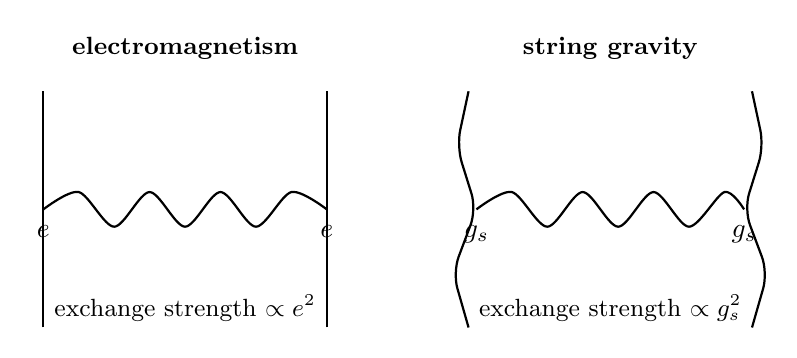
\begin{tikzpicture}[x=1cm,y=1cm]
  \node[font=\small\bfseries] at (1.8,3.55) {electromagnetism};
  \draw[line width=0.8pt] (0,0) -- (0,3);
  \draw[line width=0.8pt] (3.6,0) -- (3.6,3);
  \draw[line width=0.8pt] plot[smooth] coordinates {(0,1.5) (0.45,1.72) (0.9,1.28) (1.35,1.72) (1.8,1.28) (2.25,1.72) (2.7,1.28) (3.15,1.72) (3.6,1.5)};
  \node[below] at (0,1.42) {\(e\)};
  \node[below] at (3.6,1.42) {\(e\)};
  \node[font=\small] at (1.8,0.25) {exchange strength \(\propto e^2\)};
  \node[font=\small\bfseries] at (7.2,3.55) {string gravity};
  \draw[line width=0.8pt,rounded corners=6pt] (5.4,0) -- (5.2,0.7) -- (5.5,1.5) -- (5.25,2.3) -- (5.4,3);
  \draw[line width=0.8pt,rounded corners=6pt] (9,0) -- (9.2,0.7) -- (8.9,1.5) -- (9.15,2.3) -- (9,3);
  \draw[line width=0.8pt] plot[smooth] coordinates {(5.5,1.5) (5.95,1.72) (6.4,1.28) (6.85,1.72) (7.3,1.28) (7.75,1.72) (8.2,1.28) (8.65,1.72) (8.9,1.5)};
  \node[below] at (5.5,1.42) {\(g_s\)};
  \node[below] at (8.9,1.42) {\(g_s\)};
  \node[font=\small] at (7.2,0.25) {exchange strength \(\propto g_s^2\)};
\end{tikzpicture}
\caption{L’analogie pour le décompte des couplages. Chaque extrémité du quantum échangé contribue un facteur d’interaction.}
\end{figure}

Cette observation permet de déterminer presque entièrement la constante de Newton. Le couplage \(g_s\) est sans dimension, tandis qu’en quatre dimensions \(G_N\) a les dimensions du carré d’une longueur. La longueur microscopique disponible est \(\ell_s\) ; on a donc
\begin{equation}
G_N\sim g_s^2\ell_s^2.
\label{eq:l06-newton-string}
\end{equation}
En combinant cela avec l’équation~\eqref{eq:l06-planck-area}, on obtient
\begin{equation}
\ell_p\sim g_s\ell_s.
\label{eq:l06-planck-string}
\end{equation}

\begin{figure}[htbp]
\centering
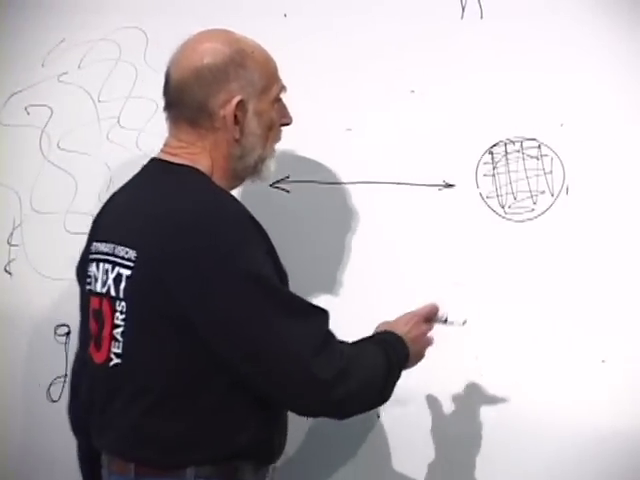
\includegraphics[width=0.72\textwidth]{lecture_06_figure_04.png}
\caption{Les relations fondamentales conservées au tableau : \(\ell_p^2=G_N\) et \(\ell_p\sim g_s\ell_s\).}
\lectureframe{00:15:45.000}
\end{figure}

L’équation~\eqref{eq:l06-newton-string} est la relation simplifiée utilisée tout au long de ce cours.\editorialnote{Dans une théorie des cordes compactifiée, la constante de Newton effective en quatre dimensions dépend également du volume de compactification et de conventions d’ordre unité. Le cours néglige ces éléments pour isoler le comportement d’échelle de la correspondance.}

\begin{classroomqa}
\audiencequestion{Le couplage \(g_s\) est-il supérieur ou inférieur à un, et quelle longueur est la plus grande ?\lecturetimestamp{00:16:00}}
\lecturerresponse{Nous travaillons à faible couplage, \(g_s<1\). Alors, d’après \(\ell_p\sim g_s\ell_s\), la longueur de corde est supérieure à la longueur de Planck. Le fort couplage exige une autre description, dont nous n’avons pas besoin ici.}
\end{classroomqa}

\section{Le dénombrement des états du trou noir}

En omettant la constante de Boltzmann et les facteurs numériques, l’entropie de Bekenstein--Hawking s’écrit
\begin{equation}
S_{\mathrm{BH}}=\frac{A}{4G_N}sim\frac{A}{G_N}sim\frac{A}{\ell_p^2}.
\label{eq:l06-bh-area}
\end{equation}
Le facteur \(1/4\) est exact dans la formule semi-classique, mais il n’intervient pas dans cet argument d’échelle.

\begin{classroomqa}
\audiencequestion{L’indice ``BH'' signifie-t-il « trou noir » ou « Bekenstein--Hawking » ?\lecturetimestamp{00:16:51}}
\lecturerresponse{Pour notre propos, il peut nous rappeler les deux. L’essentiel est que l’entropie est l’aire de l’horizon mesurée en aires de Planck.}
\end{classroomqa}

Pour un trou noir de Schwarzschild en quatre dimensions,
\begin{equation}
R_s=2G_NM,
\qquad
A=4\pi R_s^2.
\end{equation}
En omettant \(2\) et \(4\pi\), comme le fait le cours,
\begin{align}
S_{\mathrm{BH}}
&\sim \frac{R_s^2}{G_N}
\sim \frac{(G_NM)^2}{G_N} \\
&\sim M^2G_N
\sim M^2\ell_p^2.
\label{eq:l06-bh-mass}
\end{align}
C’est cette forme que nous comparerons au dénombrement des états de corde.

\section{Une corde longue comme marche aléatoire}

Partons d’une petite corde et injectons-y de l’énergie. Une corde générique très excitée ne reste pas une boucle bien ordonnée. Elle devient un objet long et emmêlé, comme du fil de pêche après un moulinet sérieusement enchevêtré. Cet enchevêtrement a une entropie, car un très grand nombre de configurations se ressemblent à l’échelle macroscopique.

Pour les dénombrer, remplaçons l’espace par un réseau dont les arêtes ont une longueur \(\ell_s\). Les sites sont les sommets, les arêtes sont les segments et les carrés élémentaires sont les plaquettes. Une corde est représentée par une suite connexe d’arêtes. Ce modèle est volontairement grossier, mais le nombre exponentiel d’états qu’il donne reproduit le comportement d’échelle recherché.

\begin{figure}[htbp]
\centering
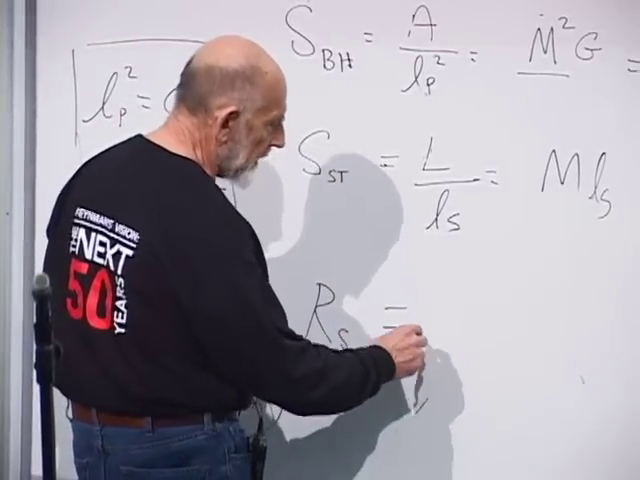
\includegraphics[width=0.72\textwidth]{lecture_06_figure_05.png}
\caption{Le modèle de réseau bidimensionnel. Le segment bleu représente un pas de la corde ; les quatre prolongements possibles sont comptés à chaque site.}
\lectureframe{00:23:50.000}
\end{figure}

\begin{classroomqa}
\audiencequestion{Combien de choix le modèle de marche simplifié offre-t-il à chaque pas ?\lecturetimestamp{00:22:43}}
\lecturerresponse{Quatre sur le réseau carré, puisque le retour immédiat en arrière est autorisé. En trois dimensions, il y en aurait six. Un autre réseau modifierait ce nombre ordinaire, mais le nombre de marches croîtrait toujours exponentiellement avec le nombre d’arêtes.}
\end{classroomqa}

Si la corde comporte \(n\) arêtes, le nombre d’états dans le modèle bidimensionnel est
\begin{equation}
\Omega_n\sim4^n.
\label{eq:l06-walk-count}
\end{equation}Il existe une marche rectiligne exceptionnelle, mais elle ne représente qu’un état parmi \(4^n\). Une marche typique se replie à plusieurs reprises et occupe une boule enchevêtrée. Pour un grand \(n\), presque toutes les configurations générées au hasard se ressemblent qualitativement.

L’entropie est le logarithme du nombre de configurations indiscernables à l’échelle macroscopique :
\begin{equation}
S_{\mathrm{st}}=\log\Omega_n\sim n\log4\sim n.
\label{eq:l06-string-entropy-n}
\end{equation}

\begin{classroomqa}
\audiencequestion{Pourquoi l’entropie est-elle proportionnelle à \(n\) plutôt qu’à \(4^n\) ?\lecturetimestamp{00:25:39}}
\lecturerresponse{L’entropie est le logarithme du nombre d’états. Ainsi, \(\log(4^n)=n\log4\), et le facteur \(\log4\) est une constante d’ordre unité que nous négligerons.}
\end{classroomqa}

Si \(L\) désigne la longueur de contour, obtenue en suivant la corde d’une extrémité à l’autre, alors
\begin{equation}
n=\frac{L}{\ell_s},
\qquad
S_{\mathrm{st}}\sim\frac{L}{\ell_s}.
\label{eq:l06-string-entropy-length}
\end{equation}
Ici, \(L\) ne désigne pas le diamètre de la boule enchevêtrée. C’est une distance bien plus grande, mesurée le long de la corde.

Passons ensuite de la longueur de contour à la masse. Avec \(c=\hbar=1\), la masse a les dimensions de l’inverse d’une longueur. Une arête de la taille d’une corde porte donc une masse de l’ordre de
\begin{equation}
m_{\mathrm{link}}\sim\frac{1}{\ell_s}.
\label{eq:l06-link-mass}
\end{equation}

\begin{classroomqa}
\audiencequestion{Pourquoi la masse d’une arête doit-elle être proportionnelle à \(1/\ell_s\) ?\lecturetimestamp{00:29:20}}
\lecturerresponse{Dans ces unités, la masse est l’inverse d’une longueur, et \(\ell_s\) est la seule longueur disponible. De façon équivalente, une tension de corde de l’ordre de \(1/\ell_s^2\), multipliée par la longueur d’une arête \(\ell_s\), donne le même résultat.}
\end{classroomqa}

La corde entière a alors
\begin{equation}
M\sim n m_{\mathrm{link}}
\sim\frac{n}{\ell_s}
\sim\frac{L}{\ell_s^2},
\qquad
L\sim M\ell_s^2.
\label{eq:l06-string-mass}
\end{equation}En substituant dans l’équation~\eqref{eq:l06-string-entropy-length}, on obtient
\begin{equation}
S_{\mathrm{st}}\sim M\ell_s.
\label{eq:l06-string-entropy-mass}
\end{equation}Le modèle de marche sur réseau néglige les contraintes de la surface d’univers et les coefficients numériques, mais la croissance exponentielle du spectre d’une corde très excitée donne le même comportement dominant.\editorialnote{La construction par marche aléatoire est un aide-mémoire pour la densité des états de corde à grand niveau d’excitation, et non une discrétisation littérale d’une corde fondamentale.}

\section{Le décalage qui amorce l’argument}

Nous avons maintenant les deux résultats :
\begin{equation}
S_{\mathrm{BH}}\sim M^2\ell_p^2,
\qquad
S_{\mathrm{st}}\sim M\ell_s.
\label{eq:l06-two-entropies}
\end{equation}Ils se ressemblent, mais ne sont pas égaux à masse fixée et pour un couplage quelconque. L’expression de l’entropie du trou noir est quadratique en \(M\) ; celle de la corde est linéaire. On ne peut pas simplement déclarer qu’une corde chaude est un trou noir sans expliquer comment les deux régimes se rejoignent.

\begin{figure}[htbp]
\centering
\includegraphics[width=0.78\textwidth]{lecture_06_figure_06.png}
\caption{La comparaison bien visible au tableau : l’entropie du trou noir en haut, celle de la corde longue en bas, avec les relations de Planck--corde conservées à gauche.}
\lectureframe{00:33:20.000}
\end{figure}

C’est là que le cours s’est interrompu. Le suspense est utile : ce décalage ne réfute pas l’idée, il indique qu’il faut comparer le même état tout en faisant varier l’intensité de la gravitation.

\section{Faire varier le couplage}

Fixons \(\ell_s\) et imaginons que \(g_s\) puisse varier. Pour \(g_s=0\), les cordes ne se scindent ni ne fusionnent, et la gravitation disparaît puisque \(G_N\sim g_s^2\ell_s^2\). Un état suffisamment énergétique est alors une corde longue et faiblement interactive.

Augmentons lentement \(g_s\). Les interactions entre cordes deviennent possibles et, ce qui importe davantage dans l’argument présent, la gravitation se renforce.

\begin{classroomqa}
\audiencequestion{Quand \(g_s\) augmente, le premier effet est-il simplement que la corde se scinde en cordes plus courtes ?\lecturetimestamp{00:36:29}}
\lecturerresponse{Les scissions et les fusions deviennent possibles, mais fixons \(\ell_s\) et suivons l’état de forte entropie. L’effet central est que \(G_N\) augmente, si bien que l’auto-gravitation de la corde longue attire vers l’intérieur la boule enchevêtrée.}
\end{classroomqa}

L’objet se contracte et devient plus dense. Son énergie potentielle gravitationnelle est négative ; la contraction abaisse donc son énergie totale et, par conséquent, sa masse.

\begin{classroomqa}
\audiencequestion{L’énergie augmente-t-elle ou diminue-t-elle lorsque l’auto-gravitation rapproche les parties de la corde ?\lecturetimestamp{00:37:48}}
\lecturerresponse{Elle diminue. L’énergie de liaison devient plus négative. La masse peut varier au cours de cette évolution, même si nous continuons à suivre le même état.}
\end{classroomqa}

À terme, la taille de l’objet devient comparable à son rayon de Schwarzschild. Au-delà de ce point, la description en termes de trou noir devient naturelle. Une excitation initiale plus importante atteint cette condition à un couplage plus faible, car un objet plus massif nécessite moins d’intensité gravitationnelle pour former un horizon.

\begin{figure}[htbp]
\centering
\resizebox{0.95\linewidth}{!}{%
\begin{tikzpicture}[x=1cm,y=1cm,>=Latex]
  \draw[->,line width=0.9pt] (0,0) -- (11,0) node[right] {increasing \(g_s\)};
  \node[draw,rounded corners,align=center,minimum width=2.6cm,minimum height=1.15cm] at (1.8,1.5) {long excited string\\weak self-gravity};
  \node[draw,rounded corners,align=center,minimum width=2.6cm,minimum height=1.15cm] at (5.5,1.5) {correspondence point\\\(R_s\sim\ell_s\)};
  \node[draw,circle,align=center,minimum size=1.8cm] at (9.3,1.5) {black\\hole};
  \draw[->,line width=0.8pt] (3.15,1.5) -- (4.1,1.5) node[midway,above,font=\small] {contracts};
  \draw[->,line width=0.8pt] (6.9,1.5) -- (8.25,1.5);
  \node[font=\small,align=center] at (5.5,-0.65) {same family of states followed slowly;\\binding energy and mass may change};
\end{tikzpicture}
}
\caption{Le parcours de correspondance à \(\ell_s\) fixée. Inverser la flèche ramène l’état de trou noir à un état de corde longue.}
\end{figure}

\begin{classroomqa}
\audiencequestion{Faut-il imaginer \(g_s\) entre zéro et un ?\lecturetimestamp{00:40:18}}
\lecturerresponse{Oui. L’argument reste dans le régime de faible couplage. Si \(g_s\) est très petit, l’état doit être d’autant plus massif pour devenir un trou noir. Nous n’avons pas besoin d’entrer dans le régime \(g_s>1\), mal contrôlé.}
\end{classroomqa}

Dans cette expérience de pensée, la variation lente est réversible.

\begin{classroomqa}
\audiencequestion{Si l’on réduit de nouveau le couplage jusqu’à ce que la gravitation ne puisse plus maintenir le trou noir, en quoi se transforme-t-il ?\lecturetimestamp{00:41:37}}
\lecturerresponse{En une corde longue. Lorsque la gravitation s’annule, tout ce qui intervient dans cette construction doit être décrit en termes d’états de corde. En faisant varier le couplage dans un sens, on passe de la corde au trou noir ; dans l’autre, du trou noir à la corde.}
\end{classroomqa}

À énergie totale et volume fixés, la configuration dominante de forte entropie est essentiellement une corde longue, plutôt qu’un très grand nombre de cordes courtes. Ce résultat n’est pas démontré ici. Il découle de la mécanique statistique des cordes près du régime de Hagedorn et nous y reviendrons.

\section{Ce que voit un observateur extérieur}

Où se trouve la corde lorsque l’objet est décrit comme un trou noir ? Dans la description extérieure, elle ne disparaît pas brusquement. En temps de Schwarzschild, le franchissement apparent est repoussé à un temps arbitrairement lointain ; les degrés de liberté de corde sont donc représentés comme s’accumulant sur l’horizon ou à proximité.

\begin{figure}[htbp]
\centering
\includegraphics[width=0.72\textwidth]{lecture_06_figure_07.png}
\caption{Comparaison au tableau entre un horizon macroscopique, où la structure à l’échelle de la corde forme une mince couche floue, et un horizon plus petit dont le rayon approche l’échelle de la boucle.}
\lectureframe{00:45:30.000}
\end{figure}

Pour \(R_s\gg\ell_s\), le trou noir est macroscopique et la structure à l’échelle de la corde ne forme qu’une mince couche par rapport au rayon de l’horizon. À mesure que le rayon diminue vers \(\ell_s\), la distinction entre un trou noir lisse et une corde étendue perd son sens. Il s’agit d’une description depuis l’extérieur, en termes d’horizon étiré ; il ne faut pas la confondre avec l’affirmation indépendante des coordonnées selon laquelle la matière en chute ne franchirait jamais un horizon régulier.\editorialnote{Le cours utilise la description extérieure familière dans le cadre de la complémentarité des trous noirs. L’expression ``sur l’horizon''désigne les degrés de liberté résolus dans la description extérieure ; elle ne constitue pas une dérivation distincte de leur position covariante.}

Le passage d’un régime à l’autre se produit lorsque
\begin{equation}
R_s\sim\ell_s.
\label{eq:l06-correspondence-radius}
\end{equation}En dessous de l’échelle de corde, la géométrie de Schwarzschild ne peut pas résoudre la structure censée la soutenir. Les boucles fluctuent hors de l’horizon éventuel, et il vaut mieux appeler corde l’état obtenu.

\section{Le point de correspondance}

Utilisons \(R_s\sim G_NM\) dans l’équation~\eqref{eq:l06-correspondence-radius} :
\begin{equation}
G_NM\sim\ell_s.
\end{equation}Substituons ensuite \(G_N\sim g_s^2\ell_s^2\) :
\begin{equation}
M g_s^2\ell_s^2\sim\ell_s,
\qquad
M g_s^2\ell_s\sim1.
\label{eq:l06-correspondence-condition}
\end{equation}

\begin{figure}[htbp]
\centering
\includegraphics[width=0.72\textwidth]{lecture_06_figure_08.png}
\caption{Le calcul complet de la transition au tableau : \(R_s\sim\ell_s\) mène à la condition sans dimension encadrée \(Mg_s^2\ell_s\sim1\).}
\lectureframe{00:49:50.000}
\end{figure}

Un membre de l’auditoire a remarqué ce que cette condition annonce. Au point de correspondance,
\begin{align}
S_{\mathrm{BH}}
&\sim M^2\ell_p^2
\sim M^2g_s^2\ell_s^2 \\
&=(M\ell_s)(Mg_s^2\ell_s)
\sim M\ell_s
\sim S_{\mathrm{st}}.
\label{eq:l06-entropy-preview}
\end{align}

\begin{classroomqa}
\audiencequestion{Les équations impliquent-elles déjà que les entropies du trou noir et de la corde deviennent égales ?\lecturetimestamp{00:50:18}}
\lecturerresponse{Oui. C’est exactement là que mène le calcul. Les éléments nécessaires ont été inscrits au tableau, mais le cours en reporte l’assemblage complet afin de revoir soigneusement le raisonnement de la correspondance.}
\end{classroomqa}

L’équation~\eqref{eq:l06-entropy-preview} donne en une ligne l’aperçu algébrique implicite dans l’échange. Elle établit le comportement d’échelle, mais pas le coefficient exact \(1/4\). Pour obtenir une égalité microscopique exacte, il faut des trous noirs mieux contrôlés et des constructions de cordes plus détaillées.\editorialnote{Le cours s’arrête avant de présenter l’équation~\eqref{eq:l06-entropy-preview} comme une dérivation complète. Elle est écrite ici parce que l’auditoire énonce explicitement l’égalité et que toutes les relations nécessaires ont déjà été introduites.}

\section{Pourquoi l’entropie se conserve au cours du passage}

Supposons qu’un paramètre de contrôle, tel qu’un champ magnétique ou \(g_s\), varie suffisamment lentement tandis que le système est isolé et que l’évolution est réversible. L’énergie, la taille et l’énergie de liaison peuvent changer, mais l’entropie est conservée :
\begin{equation}
\Delta S=0.
\label{eq:l06-adiabatic-entropy}
\end{equation}Le cours relie cela à la conservation de l’information. L’entropie mesure l’information masquée par une description à gros grains ; une variation lente et réversible du Hamiltonien réorganise les états sans effacer cette information.

\begin{classroomqa}
\audiencequestion{La conservation de l’entropie exige-t-elle que le parcours évite une transition de phase ?\lecturetimestamp{00:54:01}}
\lecturerresponse{Oui, il faut pouvoir suivre l’état de façon continue. Un système fini ne connaît pas de transition de phase thermodynamique strictement non analytique comme celle d’un système de volume infini ; si la variation est suffisamment lente, la correspondance peut être traitée comme un croisement continu.}
\end{classroomqa}

Le terme « adiabatique » est employé ici au sens plus fort de quasistatique et réversible. Un processus adiabatique mais irréversible peut produire de l’entropie ; la lenteur et la possibilité de suivre l’état sont essentielles.\editorialnote{L’énoncé thermodynamique \(\Delta S=0\) exige un parcours adiabatique réversible. En mécanique quantique, l’idée correspondante consiste à suivre le même ensemble d’états lorsque le paramètre varie, sans transitions incontrôlées entre niveaux.}

\begin{classroomqa}
\audiencequestion{Pourquoi une corde longue aurait-elle plus d’entropie que plusieurs cordes plus courtes de même masse totale ?\lecturetimestamp{00:54:44}}
\lecturerresponse{C’est contre-intuitif, mais le dénombrement explicite des états à haute énergie favorise une composante de corde longue dans un volume fixé. La démonstration est reportée ; pour l’argument présent, il nous suffit que le trou noir corresponde au secteur de cordes d’entropie maximale, plutôt qu’à un gaz dilué d’un très grand nombre de cordes courtes.}
\end{classroomqa}

La stratégie opératoire est donc la suivante :
\begin{enumerate}
\item Partir d’un trou noir de masse \(M_0\) et de couplage \(g_{s,0}\).
\item Diminuer lentement \(g_s\) tout en suivant la même famille d’états de forte entropie.
\item S’arrêter à \(R_s\sim\ell_s\), là où la description en termes de trou noir devient une description en termes de corde longue.
\item Dénombrer les états de corde à l’aide de \(S_{\mathrm{st}}\sim M\ell_s\).
\item Reporter cette entropie le long du parcours réversible jusqu’au trou noir initial.
\end{enumerate}

\begin{figure}[htbp]
\centering
\includegraphics[width=0.72\textwidth]{lecture_06_figure_09.png}
\caption{Le principe conservé au tableau pendant l’énoncé de la stratégie : une variation adiabatique de \(g_s\) ne modifie pas \(S\).}
\lectureframe{00:56:40.000}
\end{figure}

La théorie des cordes a permis d’obtenir des dénombrements d’entropie beaucoup plus précis pour les trous noirs chargés, en rotation, supersymétriques, presque extrémaux et de dimension supérieure. La discussion du trou noir neutre de Schwarzschild présentée ici est un argument de correspondance sommaire : elle établit la densité paramétrique des états et le passage physique d’un régime à l’autre, mais pas une dégénérescence protégée exacte.\editorialnote{L’accord exact est le plus solide pour les trous noirs particuliers dont le dénombrement des états reste protégé lorsque le couplage varie. Ce cours présente volontairement la version la plus simple, à l’ordre de grandeur près.}

\begin{classroomqa}
\audiencequestion{Lorsque la gravitation est coupée, l’état peut-il devenir deux cordes plutôt qu’exactement une ?\lecturetimestamp{00:58:25}}
\lecturerresponse{La probabilité d’obtenir un petit nombre de cordes longues est finie, et en utiliser deux au lieu d’une ne change pas le comportement dominant de l’entropie. Ce qui modifierait l’argument serait une fragmentation en un vaste gaz de cordes courtes ; le dénombrement statistique à haute énergie ne favorise pas cette issue.}
\end{classroomqa}

Le trou noir représente l’entropie maximale que l’on puisse concentrer dans une région ; lorsque la gravitation est supprimée, la corde longue est l’état correspondant de forte entropie. Ces deux descriptions sont désormais reliées, mais le calcul n’est pas encore développé avec précision. L’étape suivante consiste à reprendre soigneusement l’algèbre et à examiner jusqu’où l’on peut se fier à cette correspondance.
